\documentclass[11pt,letterpaper]{article}
\PassOptionsToPackage{hyphens}{url}
\usepackage[margin=.83in,top=.8in,bottom=.8in,headheight=15pt]{geometry}
\usepackage[T1]{fontenc}
\usepackage{lmodern,amsmath,amssymb,mathtools,bm,booktabs,array,graphicx,tikz}
\usetikzlibrary{arrows.meta,positioning,calc,decorations.pathreplacing,patterns}
\definecolor{ink}{HTML}{17344D}\definecolor{accent}{HTML}{087E8B}\definecolor{pale}{HTML}{EDF5F5}\definecolor{gold}{HTML}{AD6B19}
\providecommand{\dd}{\,\mathrm{d}}\providecommand{\R}{\mathbb{R}}
\providecommand{\E}{\mathbb{E}}\providecommand{\Var}{\operatorname{Var}}
\providecommand{\Cov}{\operatorname{Cov}}\providecommand{\diag}{\operatorname{diag}}
\providecommand{\norm}[1]{\left\lVert#1\right\rVert}
\providecommand{\abs}[1]{\left|#1\right|}
\usepackage{microtype,hyperref,fancyhdr,enumitem,amsthm,sectsty,needspace}
\allsectionsfont{\raggedright}
\hypersetup{colorlinks=true,linkcolor=ink,urlcolor=accent,pdfauthor={Zan Ahmad},pdftitle={Resistance networks: constitutive laws, pressure, and conservation / Lecture notes}}
\setlength{\parindent}{0pt}\setlength{\parskip}{6pt}\linespread{1.07}
\setlist{itemsep=3pt,topsep=4pt,leftmargin=*}
\emergencystretch=2em\clubpenalty=10000\widowpenalty=10000
\pagestyle{fancy}\fancyhf{}\fancyhead[L]{\small Mathematical Modeling}\fancyhead[R]{\small Lecture 2}
\fancyfoot[L]{\footnotesize Zan Ahmad}\fancyfoot[R]{\footnotesize\thepage}\renewcommand{\headrulewidth}{.3pt}
\newtheorem{proposition}{Proposition}\newtheorem{theorem}{Theorem}\newtheorem{lemma}{Lemma}
\theoremstyle{definition}\newtheorem{definition}{Definition}\newtheorem{example}{Example}
\numberwithin{equation}{section}
\begin{document}
{\small\scshape Mathematical Modeling\hfill Lecture 2}\par\medskip
{\raggedright\hyphenpenalty=10000\exhyphenpenalty=10000\LARGE\bfseries\color{ink} Resistance networks: constitutive laws, pressure, and conservation\par}\medskip
{\small Lecture notes}\par\bigskip
Conservation constrains how flows fit together but does not determine them. A constitutive relation supplies the missing connection between pressure difference and flow. We combine linear resistance laws with nodal conservation, derive the resulting matrix problem, and solve a five-link example. Signs, boundary conditions, and a positivity argument explain why the answer is determined. These arguments also produce checks that do not merely repeat the linear solve.

\section{Linear resistance is a local constitutive assumption}
\hypertarget{note-linear-resistance-is-a-local-constitutive-assumption}{}\label{note:linear-resistance-is-a-local-constitutive-assumption}
{\small \href{slides.html\#frame=conservation-needs-a-constitutive-law\&step=1}{Slides for this section}}\par
For an open link joining nodes $i$ and $j$, choose positive flow from $i$ to $j$ and write
\[
Q_{i\to j}=G_{ij}(P_i-P_j),\qquad G_{ij}=R_{ij}^{-1}>0.
\]
Pressure is measured in mmHg, flow in L/min, resistance in $\mathrm{mmHg}\,\mathrm{min}/\mathrm L$, and conductance in $\mathrm L/(\mathrm{min}\,\mathrm{mmHg})$. A negative $Q_{i\to j}$ means flow opposite the reference arrow. Reversing the arrow reverses the signed variable and its pressure difference, while preserving the physical flow.

The law represents a dissipative link with a fixed linear response. It does not represent a valve: an open resistor allows either direction. It also excludes storage within the link and ignores inertial transients, diameter changes, collapse, and pressure-dependent material response. The volume-storage relation $V=V_d+CP$ is a different constitutive law. A resistor determines a flow from a pressure difference; a compliance determines stored volume from a distending pressure.

The link dissipates mechanical power proportional to
\[
(P_i-P_j)Q_{i\to j}=G_{ij}(P_i-P_j)^2=R_{ij}Q_{i\to j}^{2}\geq0.
\]
The expression has pressure times volume per time units; a conversion is required to report watts. Negative signed flow does not imply negative dissipation.
\section{Boundary pressures are data; interior pressures are unknowns}
\hypertarget{note-boundary-pressures-are-data-interior-pressures-are-unknowns}{}\label{note:boundary-pressures-are-data-interior-pressures-are-unknowns}
{\small \href{slides.html\#frame=prescribed-endpoints-and-unknown-interiors-figure\&step=1}{Slides for this section}}\par
Use two prescribed endpoint pressures, $P_H=96$ and $P_L=6\ \mathrm{mmHg}$. The interior nodes are $A$ and $B$. Their links have resistances
\[
R_{HA}=20,\quad R_{AL}=10,\quad R_{HB}=10,\quad R_{BL}=20,\quad R_{AB}=20
\]
in $\mathrm{mmHg}\,\mathrm{min}/\mathrm L$. The bridge arrow is $A\to B$. Prescribed endpoints may be maintained by external pumps or reservoirs; they are not unknowns solved by conservation at $A$ and $B$.

At a non-storing interior node, total inflow equals total outflow. Combining that statement with the constitutive law gives
\begin{align*}
0&=\frac{96-P_A}{20}-\frac{P_A-6}{10}-\frac{P_A-P_B}{20},\\
0&=\frac{96-P_B}{10}+\frac{P_A-P_B}{20}-\frac{P_B-6}{20}.
\end{align*}
The bridge occurs with opposite signs. These equations would instead have $\dot V_A$ and $\dot V_B$ on the left in a model with storage. Steady flow is an approximation imposed here, not a general property of vessels.
\begin{center}\begin{minipage}{.98\linewidth}\centering
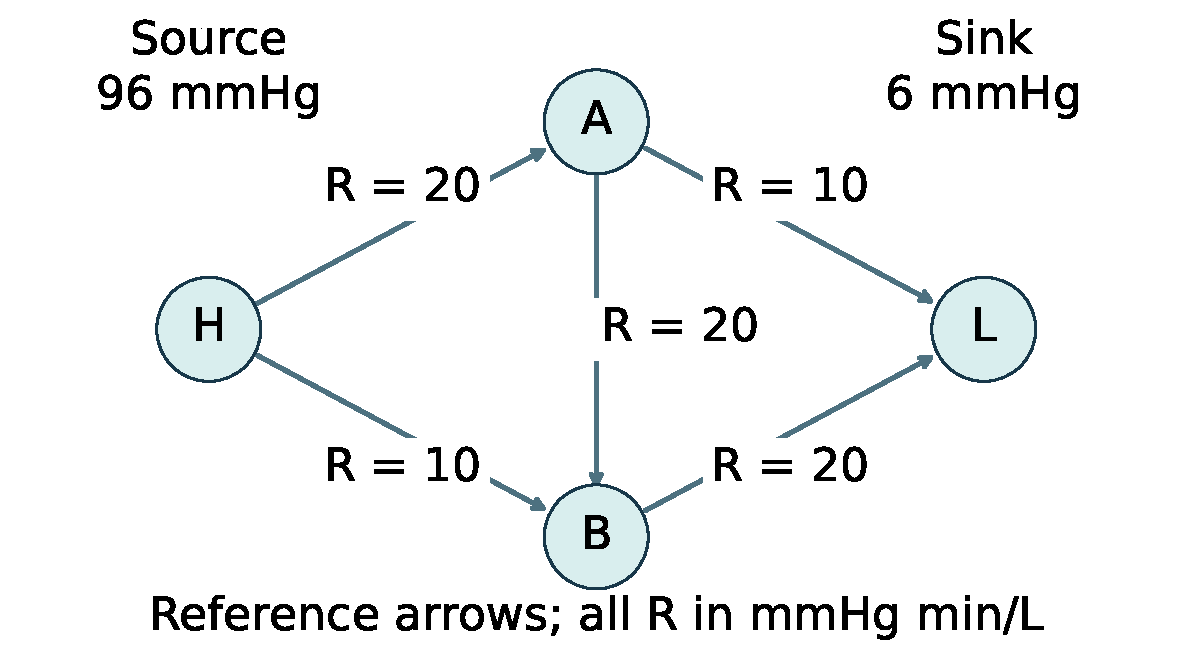
\includegraphics[width=.96\linewidth,height=.57\textheight,keepaspectratio]{presentation-figures/network.pdf}\par\smallskip
{\small Original synthetic network. Endpoint pressures are fixed; internal pressures follow from conservation. Arrows declare reference directions, and every link is an open resistor.}
\end{minipage}\end{center}
\section{Solve the two unknowns, then recover every flow}
\hypertarget{note-solve-the-two-unknowns-then-recover-every-flow}{}\label{note:solve-the-two-unknowns-then-recover-every-flow}
{\small \href{slides.html\#frame=collect-and-eliminate\&step=1}{Slides for this section}}\par
Multiply both equations by the resistance unit value $20$ and collect unknown pressures:
\[
4P_A-P_B=108,\qquad -P_A+4P_B=198.
\]
The coefficients arise from the conductances incident on each node. Eliminating $P_B$ gives $15P_A=630$, hence
\[
\boxed{P_A=42\ \mathrm{mmHg},\qquad P_B=60\ \mathrm{mmHg}.}
\]
Substitution into the five local laws gives
\[
\begin{array}{c|rrrrr}
\text{reference link}&H\to A&A\to L&H\to B&B\to L&A\to B\\\hline
Q\ (\mathrm L/\mathrm{min})&2.7&3.6&3.6&2.7&-0.9
\end{array}
\]
The actual bridge flow is $0.9\ \mathrm L/\mathrm{min}$ from $B$ to $A$. Audit $A$: $2.7-3.6-(-0.9)=0$. Audit $B$: $3.6+(-0.9)-2.7=0$. The external inlet and outlet totals both equal $6.3\ \mathrm L/\mathrm{min}$.

The effective resistance between the prescribed endpoints is $(96-6)/6.3=100/7\approx14.286\ \mathrm{mmHg}\,\mathrm{min}/\mathrm L$. It is a property of this complete network, not the resistance of a single branch.
\begin{center}\begin{minipage}{.98\linewidth}\centering
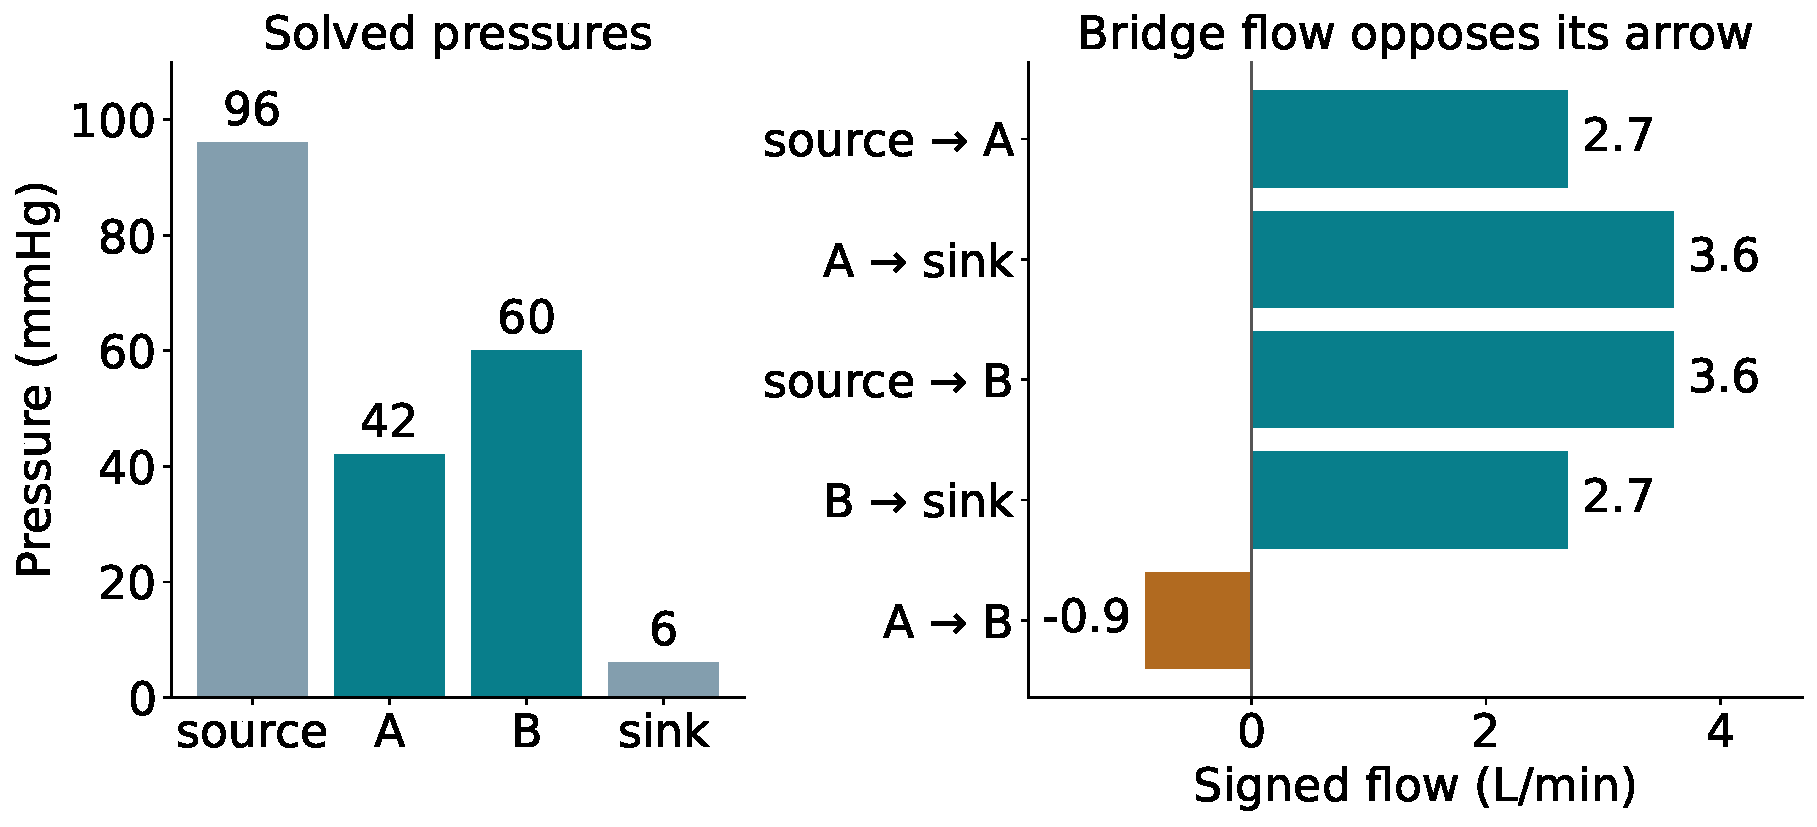
\includegraphics[width=.96\linewidth,height=.57\textheight,keepaspectratio]{presentation-figures/pressures-and-flows.pdf}\par\smallskip
{\small The solved internal pressures are 42 and 60 mmHg. Bridge flow is -0.9 L/min in the A-to-B reference, so its actual direction is B to A.}
\end{minipage}\end{center}
\section{The conductance matrix and a uniqueness argument}
\hypertarget{note-the-conductance-matrix-and-a-uniqueness-argument}{}\label{note:the-conductance-matrix-and-a-uniqueness-argument}
{\small \href{slides.html\#frame=the-graph-matrix\&step=1}{Slides for this section}}\par
For an arbitrary interior node $i$, conservation is
\[
\sum_{j\sim i}G_{ij}(P_i-P_j)=0.
\]
Move known boundary pressures to the right. If $\mathbf p$ contains the unknown interior pressures, the system is $L_{II}\mathbf p=\mathbf b$, where diagonal entries sum all incident conductances and off-diagonal entries equal $-G_{ij}$. The example is
\[
\begin{bmatrix}.20&-.05\\-.05&.20\end{bmatrix}
\begin{bmatrix}P_A\\P_B\end{bmatrix}
=\begin{bmatrix}5.4\\9.9\end{bmatrix}.
\]
The right-hand side has flow units. To see uniqueness, let $\mathbf z$ be the difference of two solutions with identical boundary values. Extend $z$ by zero at boundary nodes. Then
\[
\mathbf z^TL_{II}\mathbf z=\sum_{\{i,j\}}G_{ij}(z_i-z_j)^2.
\]
Each undirected edge is counted once. The sum can vanish only if $z$ is constant along every connected path. If every interior connected component reaches a prescribed-pressure node, that constant must be zero. Thus $L_{II}$ is positive definite and the solution is unique. An isolated component with no pressure reference instead has an undetermined additive constant.

A second consequence is the weighted-average identity
\[
P_i=\frac{\sum_{j\sim i}G_{ij}P_j}{\sum_{j\sim i}G_{ij}}.
\]
An interior pressure therefore lies between the minimum and maximum prescribed boundary pressures, under the same connectivity assumption. A result outside that range signals an error or an additional source not present in this passive model.
\section{Transformations that expose errors}
\hypertarget{note-transformations-that-expose-errors}{}\label{note:transformations-that-expose-errors}
{\small \href{slides.html\#frame=change-the-pressure-reference\&step=1}{Slides for this section}}\par
Adding one constant $c$ to every prescribed and computed pressure leaves every difference, and hence every flow, unchanged. The zero of pressure is a reference choice in this resistance-only model. This does not authorize shifting internal pressure without shifting the external pressure in a compliance law: distending pressure is itself a difference.

If every resistance is multiplied by $k>0$, every conductance is divided by $k$. Both sides of the interior matrix problem scale by $1/k$, so the interior pressures remain unchanged while every flow is divided by $k$. Doubling only one resistance is a different experiment and redistributes the pressure field.

For two links in series with no branch, conservation gives one common flow. Adding pressure drops gives $R_{\rm eq}=R_1+R_2$. For links in parallel between the same endpoints, adding flows gives $G_{\rm eq}=G_1+G_2$. These reductions apply only when the relevant topology really is series or parallel. The bridge in the five-link example prevents reducing its four outer links as two independent series paths.
\section{Computational residuals and the scope of a claim}
\hypertarget{note-computational-residuals-and-the-scope-of-a-claim}{}\label{note:computational-residuals-and-the-scope-of-a-claim}
{\small \href{slides.html\#frame=a-numerical-residual-is-necessary\&step=1}{Slides for this section}}\par
Compute pressures by a linear solve rather than forming an explicit matrix inverse. Recover each edge flow once, use that same value in both endpoint accounts, and report the residual $\mathbf r=L_{II}\mathbf p-\mathbf b$. A small residual is evidence that the assembled equations were solved, not that the correct network was assembled.

Complement it with the hand-computed five flows, equal external inlet and outlet totals, reference-pressure invariance, resistance scaling, and the interior pressure bounds. Check positive finite resistances and finite assembled coefficients; an overflow is a failed calculation, not a new physiological regime.

To test a real network, compare predicted flows with independent measurements at specified pressure boundaries. A mismatch can arise from a wrong resistance, an omitted branch, storage during a transient, or a nonlinear vessel response. The present model predicts neither pulse-wave propagation nor the contraction of the heart. It isolates a question that can be answered completely: how do prescribed endpoint pressures distribute steady flow through a passive resistive graph?
\bigskip
\section*{Exercises}
\par\noindent\begin{minipage}{\linewidth}
\subsection*{M2-1. Interpret the arrow}
An open resistor joins A at 35 mmHg to B at 50 mmHg. R=\allowbreak{}5 mmHg min/L; positive flow is defined from A toward B.

\textbf{a} Calculate the signed reference flow and its physical direction.

\end{minipage}\par\medskip
\textbf{b} Redraw the reference arrow from B toward A. What changes?

\textbf{c} Would setting the negative value to 0 preserve the stated resistor law?

\par\noindent\begin{minipage}{\linewidth}
\subsection*{M2-2. Two resistors in series}
A source at 80 mmHg connects through R1=\allowbreak{}10 mmHg min/L to node X, then through R2=\allowbreak{}5 mmHg min/L to a sink at 5 mmHg. X has no other connection and no accumulation.

\textbf{a} Explain why the two flows must be equal and calculate their value.

\end{minipage}\par\medskip
\textbf{b} Find the pressure at X and check the downstream link.

\textbf{c} If both resistances double with boundary pressures fixed, what happens?

\par\noindent\begin{minipage}{\linewidth}
\subsection*{M2-3. Audit a branch report}
A steady junction receives 7 L/min from one link and sends 2 L/min through a second. A third reference arrow points outward from the junction.

\textbf{a} Find the third signed flow required by balance.

\end{minipage}\par\medskip
\textbf{b} A report instead lists Q3=\allowbreak{}6 L/min. What accumulation rate would those three flows imply?

\textbf{c} Give two distinct possible causes of the inconsistent report and an observation that could distinguish them.

\par\noindent\begin{minipage}{\linewidth}
\subsection*{M2-4. Use an informative limiting case}
Keep the original five positive resistances but set both boundary pressures to 20 mmHg.

\textbf{a} Propose the internal pressures and all five flows.

\end{minipage}\par\medskip
\textbf{b} Verify why the node balances hold.

\textbf{c} A modified program reports nonzero circulating flow. Name one implementation check and one model change that could explain it.

\section*{References}
\noindent\begin{minipage}{\linewidth}
Zan Ahmad, Fall 2024 HEART syllabus. PDF pages 1--2.

\end{minipage}\par\medskip
\noindent\begin{minipage}{\linewidth}
Hoppensteadt and Peskin, Modeling and Simulation in Medicine and the Life Sciences, second edition. Printed pages 8--10; PDF pages 21--23 in the supplied copy.

\end{minipage}\par\medskip
\end{document}
